






% =========----------	[ Space left here for distraction free mode] ----------==========%









\subsection{Analysis 1: Does viewing position effect spatial attribute scores?}
	\label{ana1}

		% Ana1 Intro
		To assess the potential effect of viewing position on spatial attribute score, data was grouped into 8 sections: An average score for each spatial audio attribute (4 groups) each split into the average score for viewing position A and B (8 groups) illustrated in figure \ref{image:AvsB}. \\

		\begin{figure}
			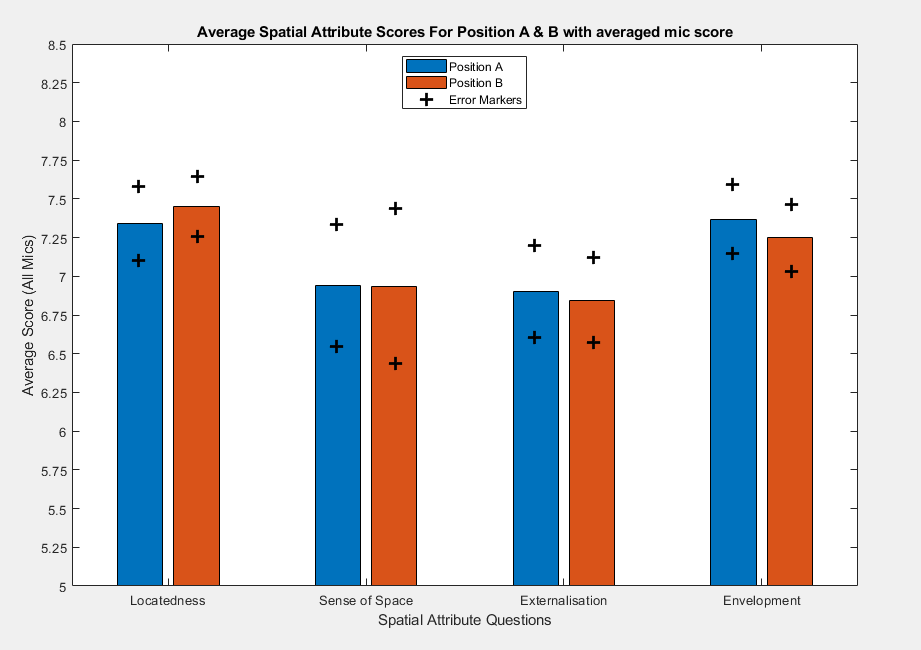
\includegraphics[width=0.5\textwidth]{images/plots/AvB_Bar_error.PNG}
			\caption{Bar chart showing average spatial attribute score for each spatial attribute at viewing position A and B}
			\label{image:AvsB} 
		\end{figure}

		It can be seen that the average spatial attribute score for viewing position A and B for each spatial attribute are close with the difference in overall mean score being 0.02. Running a Two-Sample T-Test between each of the four spatial attribute groups (e.g A vs B for locatedness etc) indicates no statistical significance. Running the same test for the averaged combined spatial attribute score (average of all four spatial attribute scores) also indicates no statistical significant between viewing position. This is made clear in figure \ref{image:AvsB_dist} illustrating the overall similarity in the distribution of scores for viewing position A and B. \\
		
		% NOTE: Should I display the distributiong as 'normal' or 'kernel'?
		\begin{figure}
			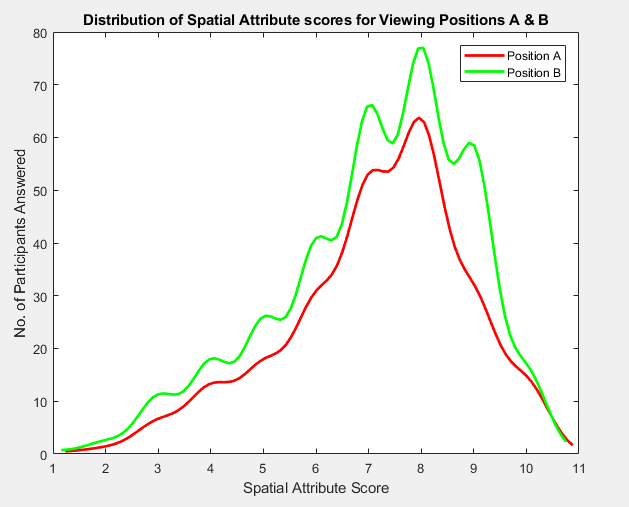
\includegraphics[width=0.5\textwidth]{images/stats/AvsB_sa_stack_all.PNG}
			\caption{Histogram showing the distribution of spatial attribute scores for viewing position A and B. This indicates that viewing position has little effect on spatial qualities in a VR environment.}
			\label{image:AvsB_dist} 
		\end{figure}

		\textbf{Conclusion}\\

		The bar chart indicates that the average spatial attribute scores are extremely close with an overall average for both being 7.1. The Two-Sample T-Test indicates that the probability of these results recurring is not unlikely ($p > \alpha (0.05)$) and therefore the results shown are not statistically significant.

